\chapter{API}

\section{Shader}

\subsection{screen space derivative}
屏幕空间偏导数
GPU always evaluate fragment/pixel shaders on 2x2 blocks of pixels at a time.

use this techniques for rendering antialiased lines

\begin{figure}[h]
    \centering
    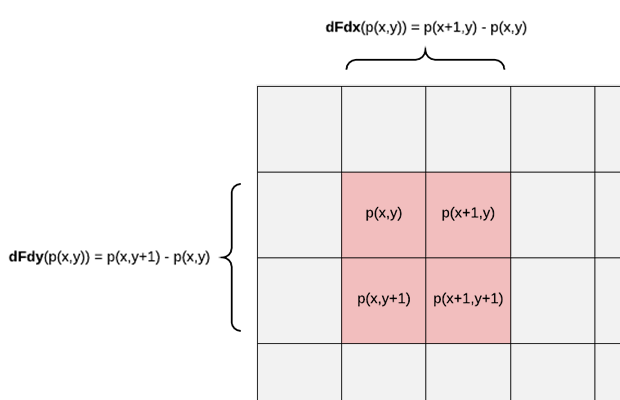
\includegraphics[width=\textwidth]{images/Shader-Derivatives.png}
\end{figure}

antialiasing,AA抗锯齿,对于一张纹理,给定UV坐标后,不仅仅是直接采样,还要考虑周围方形
区域内采样的结果,这个区域就是ddx和ddy给定的区域,在shader中调用texture时,后台进行了处理,
在一些高级的profiles中,还是允许自定义滤波窗口大小的

mipmap,在屏幕空间中,纹理坐标变换剧烈,Derivatives are used during texture sampling to
select the best mipmap level.

\subsubsection{fwidth}
GLSL中,fwidth函数返回的是X和Y方向偏导数的绝对值的和,而单方向的偏导数可以通过ddx和ddy获得

注意,这些函数与像素有关,只能在fragment/pixel shader中使用

\section{Vulkan}

vulkan是控制GPU设备的API,相比OpenGL,由OpenGL驱动提供的功能都需要自己实现,包括,同步,进度,内存管理等。
所以vulkan是适合大型复杂的图形渲染,定制性要求很高,OpenGL提供不了的功能。

\subsection{Resource}

vulkan的操作基于数据,所有data都存储在resources中,它们被后台内存管理着,构建这些资源大致有两步
\begin{itemize}
    \item {resource is created, ex, vkCreateBuffer}
    \item {resource needs to be backed by memory, 允许应用程序管理内存}
\end{itemize}

\subsubsection{buffers}

线性存储块,可拥有存储任何的数据,它同样可以存储图像数据

\subsubsection{images}

图像,具有结构性,类型,格式的固定数据

\section{3D Render Library}

\subsection{OpenSceneGraph}

\subsection{bgfx}

\subsection{three.js}

\subsection{Babylon.js}
